\documentclass[12pt]{article}

\usepackage{amsmath}
\usepackage{amssymb}
\usepackage{graphicx}
\usepackage{tikz}

\counterwithin*{equation}{section}
\counterwithin*{equation}{subsection}
\addtolength\parskip{\bigskipamount}

\graphicspath{ {./images/} } 

\begin{document}
\section{Motion in Space}

\(\vec{r} (t) =  \) position vector at time t

\(\vec{v(t)} = \vec{r}\ '(t) =  \) velocity vector at time t

\(|\vec{v} (t)| \) = speed at time t = \(|\vec{r}\ '(t)| = \frac{ds}{dt} = \) rate of change of distance with respect to time 

\(\vec{a} (t) = \vec{v}\ '(t) = \vec{r}\ ''(t)= \) acceleration vector at time t

\subsection{Motion in Space Example 1}
Let \(\vec{r} (t) = <t^2,t> \) .

Find its velocity, speed, and acceleration when \(t=1\)s.

\(\vec{v} (t) = \vec{r}\ '(t) = <2t,1> \Rightarrow \vec{v} (1) = <2,1>  \) 

Speed at \(=|\vec{v} (1) = \sqrt{2^2+1^2} = \sqrt{5} \)m/s 

\(\vec{a} (t) = \vec{v}\ '(t) = <2,0> \Rightarrow \vec{a}(1) = <2,0>   \) 

Sketch the curve \(\vec{r} (t) \) along with \(\vec{v} (1) \) and \(\vec{a} (1)   \) .

\subsection{Motion in Space Example 2}
Give \(\vec{r} (0) = <0,0,1>, \vec{v}(0) = <-1,1,1>   \), and \(\vec{a} (t) = <6t,1,4t> \)    

\underline{Aside:} \(\vec{v} (t) = \vec{v} (t_0) + \int_{t_0}^{t}\vec{a} (u)  du
  \) 

\subsection{Newton's 2nd Law}
\( \vec{F} (t) = m \vec{a} (t)\)  

\subsubsection{Newton's 2nd Law Example 1}
Uniform circular motion
\[
	\vec{r} (t) = a\cos(wt)\hat{i} + a\sin(wt)\hat{j} 
\]
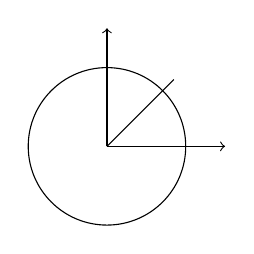
\begin{tikzpicture}
	\draw[->] (0,0) -- (1.5,0);
	\draw[->] (0,0) -- (0,1.5);
	\draw (0,0) circle (1cm);
	\draw (0,0) -- (45:1.2cm);
\end{tikzpicture}

\subsubsection{Newton's 2nd Law Example 2}
Projectiles. We fire a projectile with initial velocity \(\vec{v_0}  \) at an angle of elevation \(\alpha\). find its position function \(\vec{r} (t) \). What \(\alpha\) maximizes the range of the projectile?    

\begin{tikzpicture}[scale=2]
	\draw (0,0) -- (5,0);
	\draw (0,0) -- (0,1.5); 
\end{tikzpicture}

\subsection{Parametric Equations of the Trajectory}

\(x=(v_0\cos\alpha)t\) \\%
\(y=(v)9\sin\alpha)t - \frac{1}{2}gt^2\) 

\subsubsection{Parametric Trajectory Equations Example 1}
Our projectile is fired with a muzzle speed of 200 m/s at an angle of elevation of \(60^o\) from a position 15m above the ground.
Where does it hit the ground and with what speed?

ANSWER: \(t=-0.08\) or 35.43\\%
x = 3543m at \(200.73\) m/s
\end{document}

